\chapter{Related work and Background}
\label{ch-2}
\section{Related work}
\subsection{Gravity Spy}
The construction of one of the main datasets for the classification and detection of glitches is the Gravity Spy dataset \citep{zevin2017gravity, glanzer2023data}. 
The Gravity Spy dataset consists of a large set of Qscans (also called spectrograms). These Qscans are obtained via the Omicron algorithm pipeline \citep{robinet2020omicron}. Omicron originates from the Q-transformation \citep{chatterji2004multiresolution}. The colour scale, or normalized energy, used in these images, as in Figure \ref{fig:spectrogram_examples}, is the square of the \acrshort{snr} in a given Q-tile, divided by the mean squared magnitude for stationary white noise.
\begin{figure}[H]
    \centering
    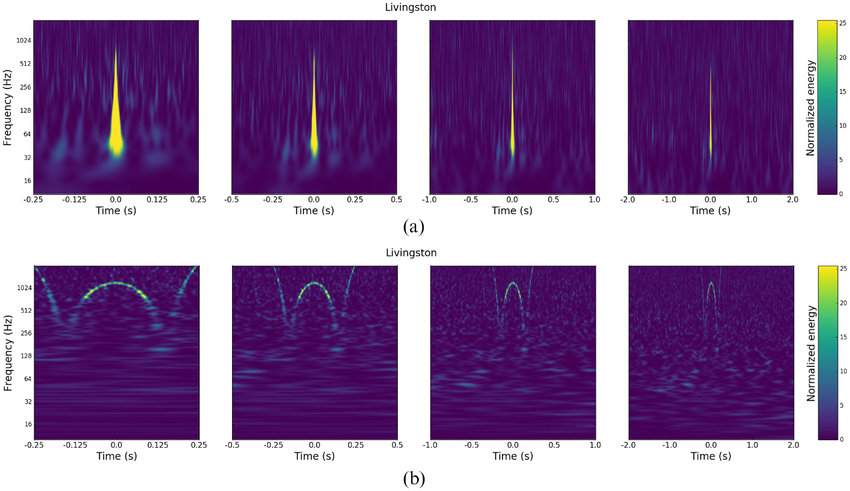
\includegraphics[width=0.8\textwidth]{Images/omegascan_examples.jpg}
    \caption{\acrshort{ligo} Qscan images of 'blip' (first row) and 'whistle' (second row) over four different durations \citep{zevin2017gravity}}
    \label{fig:spectrogram_examples}
\end{figure}
The researchers use visual inspection by citizen scientists as well as \acrshort{dl} classification using a \acrshort{cnn}. The \acrshort{cnn} outputs a confidence score $p$ for each glitch class by using a softmax layer. \\

\subsection{Glitch classification}
Because the \acrshort{gw} signal strength is weaker than the background noise, the preferred architecture is often a \acrshort{cnn}'s with wavelet and Q-transforms \cite{cuoco2020enhancing}. 

The proposed \acrshort{dl} methodology presented in \citep{bicskin2023fast} uses a combination of \acrshort{ml} and \acrshort{dl} algorithms for classification. It consists of two phases, first, they utilise feature extraction possibilities of the pre-trained \acrshort{dl} models Inception-v3 \citep{szegedy2016rethinking} and ResNet-50 \citep{he2016deep} on the Q-transformed glitch images. Secondly, they apply \acrshort{pca} to select 100 components, these serve as input for \acrshort{svm}, \acrshort{lr} and \acrshort{xgb} algorithms. They opted to use only 10 glitch classes from the Gravity Spy dataset and no up- or downsampling techniques to issue the imbalancedness of the dataset. All samples are Q-transformed before entering the training phase. The results showed that Inception-v3-based architectures perform faster and the \acrshort{lr} algorithm delivers the highest accuracy on the test set ($96.06$\%). Certain glitch morphologies like '1400 ripples', 'light modulation', 'Tomte' and 'None of the above' had substantially lower scores.

The usage of \acrshort{cnn} for glitch classification is described in \citep{fernandes2023convolutional}. They opt for a ResNet \citep{he2016deep} architecture baseline (ResNet18 and ResNet34) and the \verb|fastai| \verb|fit_one_cycle| route. 

\subsection{GW detection}
The updated Gravity Spy classification model \citep{jarov2023new} can differentiate \acrshort{cbc} signals from detector glitches. To achieve this accuracy improvement, they used a two-step approach. First, a baseline segment is selected from \acrshort{o3} and the \verb|pycbc| package \citep{nitz2020gwastro} is used to inject waveform simulations originating from masses between $3M_{\odot}$ and $350M_{\odot}$. Secondly, two classifiers (one for low-mass signals and one for high-mass \acrshort{cbc} signals) are implemented. Because certain glitch morphologies have similar structures, this type of noise must be inserted in the training set as well. Finally, the Gravity Spy CNN architecture is retrained on the extended training sets resulting in a signal-versus-glitch classifier. The relationship between the total mass of the inspiraling objects and the \acrshort{gw} accuracy was the main reason for splitting the classifiers into low and high masses. 
\subsection{Object detection for CBC}
\begin{wrapfigure}{r}{5cm}
    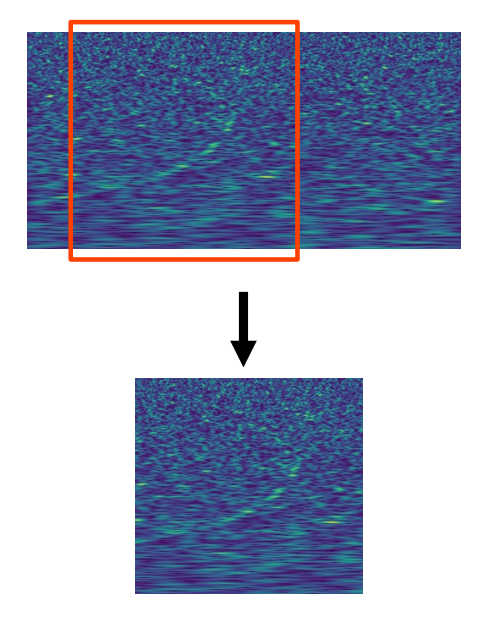
\includegraphics[width=0.25\textwidth]{Images/od_bns.png}
    \caption{Qscan generation and final 8-bit PNG image \citep{aveiro2022identification}}
    \label{fig:od_bns}
\end{wrapfigure}
Researchers \citep{aveiro2022identification} have investigated the use of a classical single shot \acrlong{od} method, \acrfull{yolo} \citep{redmon2016you}, to detect a subset of \acrshort{cbc} events, namely \acrshort{bns} mergers. Single shot detector methods are cost- and time-efficient \citep{redmon2017yolo9000} and hence are suitable candidates to integrate in a \acrshort{cbc} object detection method. 
They use generated \acrshort{bns} signals via the \verb|PyCBC| package \citep{nitz2020gwastro} and the generation pipeline from \citep{gebhard2019convolutional}. The generated signals are then randomly cut to the required 8s duration, with one condition, the generated waveform must be in the cut. 
Just as in the Gravity Spy generation process \citep{zevin2017gravity}, the Q-transform \citep{chatterji2004multiresolution} is used to generate the Qscans (here they opt for the \verb|librosa| package \citep{mcfee2015librosa}). 

The Qscans are converted to 8-bit PNG images as seen in Figure \ref{fig:od_bns}

The bounding box coordinates of the \acrshort{gw} class are included in a separate text file per image. Labelling is automated as part of the generation pipeline. Initial tests were promising with acceptable \acrfull{map} results. The research team experimented with varying \acrshort{snr} parameters (between 10 and 20). Lower \acrshort{snr} degraded the resulting metrics. Although no real training data were used, exploratory tests on GW170817 \citep{abbott2017gw170817} and GW190425 \citep{abbott2020gw190425} \acrshort{bns} coalescence events indicate the model's ability to perform \acrshort{gw} detections.



\subsection{Fractal based noise characterisation}
Two relevant studies were \citep{cavaglia2022characterization} and \citep{laguarta2023detection}. The noise found in \acrshort{gw} detectors usually is non-Gaussian and non-stationary \citep{abbott2020guide}. Distinguishing noise from spectrograms and auxiliary channels can be done straightforwardly, but determining the \acrshort{cbc} parameters is not \citep{powell2018parameter}. Researchers \citep{cavaglia2022characterization} propose utilising \acrfull{fd} on auxiliary channels like instrumental control data to identify transient origins of noise. \acrshort{fd} calculation approximations are done in a time-efficient way. Fractals are basically subsets of $n$-dimensional Euclidean spaces \citep{mandelbrot1989fractal} where $D_{F} < n$ and $D_{F} \not\in \mathbf{Z}$. \acrshort{fd} measures the degree of complexity of the set. The Minkowski-Bouligand or box-counting definition is used \citep{weisstein2019minkowski}. The definition used in \citep{cavaglia2022characterization} is taken from \citep{dubuc1989evaluating}. 
Because exact measurements are not uniformly defined, approximations like \acrfull{var} or \acrfull{anam} are used.\citep{cavaglia2022characterization} prefers the \acrshort{var} approximation and applies it to two stretches of \acrshort{ligo} data from \acrshort{o3} where whistle glitches occur. Whistle glitches are short-duration noise (around 1 second) and have a frequency between 100Hz and several kHz.  In the analysis, the focus lies on the strain data and only one auxiliary channel \verb|L1:LSC-PRCL_OUT_DQ| (interferometer PRC (Power Recycling Cavity) monitor). 
\begin{figure}[H]
    \centering
    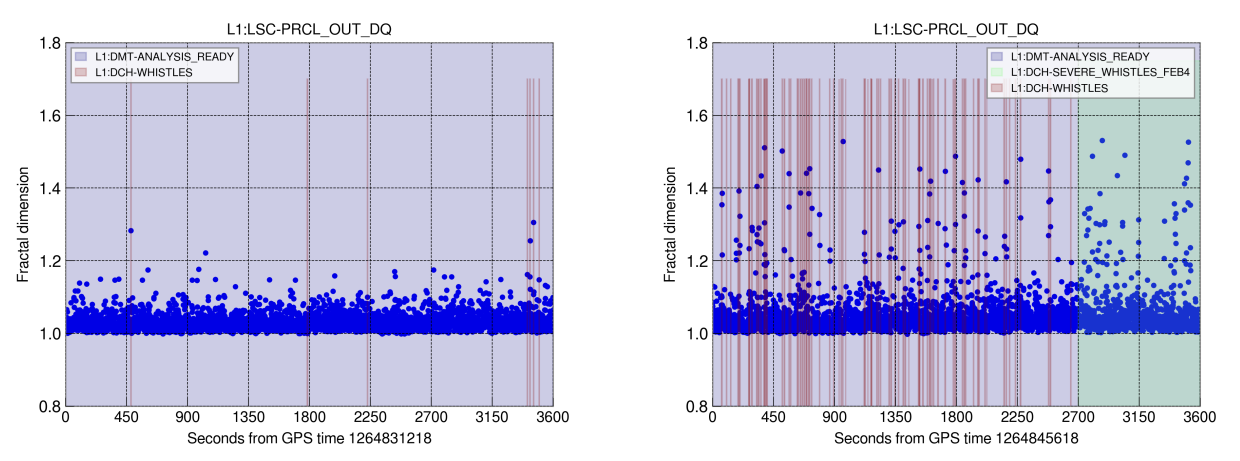
\includegraphics[width=0.9\textwidth]{Images/fd_L1_LSC_PRCL_OUT_DQ.png}
    \caption{\acrshort{fd} plot for the L1:LSC-PRCL\_OUT\_DQ auxiliary witness channel. On the left plot nominal interferometer observing mode. On the right plot data with a growing rate of glitches. \citep{cavaglia2022characterization} }
    \label{fig:fd_L1_LSC_PRCL}
\end{figure}
In the left plot of Figure \ref{fig:fd_L1_LSC_PRCL} it is clear that the nominal \acrshort{fd} is static and $D_{F}$ ranges between 1 and 1.2. Investigating the Q-scans of the noise points with $D_{F} > 1.2$ shows, at least for three out of four points, a clear whistle signal is diagnosed. In the right plot a big amount of noisy glitches is shown, this renders the data unusable for \acrshort{gw} analysis. Their experiment was done on another data strain, showing similar results. They conclude that \acrshort{fd} can be used to investigate the stationarity (or non-) of the interferometer in the company of noise.  Periods with a lot of (high) frequency noise show an increase in \acrshort{fd} variability \citep{cavaglia2022characterization}.

Researchers \citep{laguarta2023detection} use a convolutional autoencoder approach to cope with the absence of a ground truth and the absence of absolute order (variety of magnitudes). Although there are many studies on glitch morphologies, we are not sure whether the proposed class is the real class. Autoencoders have the ability to discover new structures without prior knowledge \citep{bank2023autoencoders}. The absence of absolute ordering can be tackled via the application of periodic convolutions. 
\begin{figure}
    \centering
    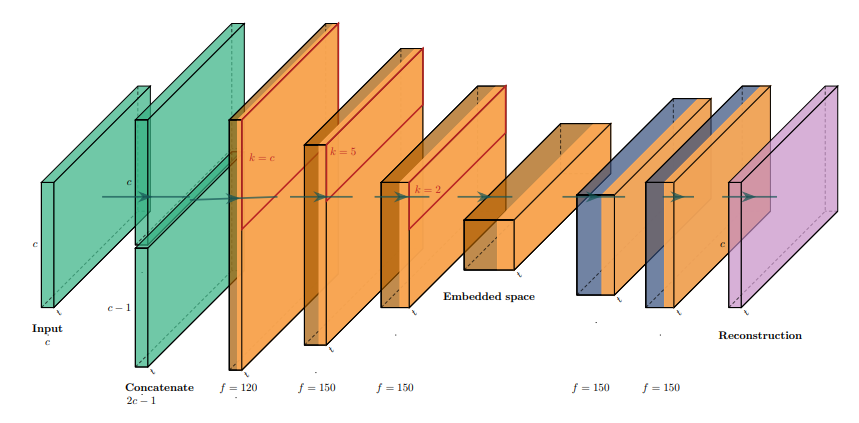
\includegraphics[width=0.8\textwidth]{Images/autoencoder_periodic_convolution.png}
    \caption{Autoencoder architecture with periodic convolutions implementation. \citep{laguarta2023detection}}
    \label{fig:autoencoder_laguarta}
\end{figure}
The autoencoder architecture is seen in Figure \ref{fig:autoencoder_laguarta}, each convolution layer is accompanied by a ReLU (Rectified Linear Unit) activation function. Despite the lowered dimensionality in the autoencoder, it is still very high. The t-SNE method can be applied for further dimensionality reduction. 
The results indicated that the autoencoder reconstruction error was highest in instances of the \verb|Scattered_Light| class. 
Safe auxiliary channel \acrshort{fd} analysis can be beneficial for noise detection and classification. Extending the proposed technique to other interferometers and investigating possible safe auxiliary channels - data strain glitch correlations is recommended.

\subsection{Glitch identification from Environmental data}
A study by \citep{colgan2020efficient} extracts useful statistical information from auxiliary channels in the vicinity of a glitch (in a 2.5 second timewindow), the acquired data is then used in a logistic regressor classifier. To limit the amount of weights, elastic net regularization \citep{zou2005regularization} is applied for penalisation. 
The results vary around 80 \% accuracy, but it does not predict the glitch class, only if it is a possible glitch or not. 

\subsection{LIGO's fourth observing run}
The initial evaluation of the fourth observing run (04) highlighted constraints in the architecture of the Gravity Spy machine learning model. Its simplicity led to challenges in generalization and the incapacity to effectively process inputs from multiple time windows \citep{wu2024advancing}. The drawbacks of the Gravity Spy classifier, as indicated in \citep{jarov2023new, alvarez2023gspynettree}, primarily include the significance of the location within the images. A line positioned at the top or bottom of the images is crucial as it represents various glitches at different frequencies. This characteristic poses difficulties for the traditional \acrshort{cnn} architecture in capturing distinctive features in glitch classes. Additionally, the shallow network structure necessitates substantial resizing of input dimensions, leading to a loss of information. Finally, the classifier struggles with an issue of confidence overfitting. In their study, researchers \citep{wu2024advancing} suggest a new architecture and compare three fusion strategies.
\newpage
\subsection{Incremental learning}
\label{ref:sub_incremental}
\subsubsection{Introduction}
In \acrshort{il} or also called \acrshort{cl}, we feed the data progressively to the model and thus acquire new knowledge over time (just as humans do). It is especially useful and efficient in learning from sequential, non-stationary data, such as wave signals. 
\citep{van2022three} illustrates the three scenarios of \acrshort{il} in terms of input $X$, context $C$ and within-context output space $Y$. 

\begin{table}[H]
\begin{tabularx}{0.9\textwidth}{l | X | l}
    \textbf{Scenario} & \textbf{Description} & \textbf{Mapping} \\
     Task-incremental learning & sequential learning of distinct task solutions. & $f:X\times C \mapsto Y$  \\
     Domain-incremental learning & Problem-solving in different contexts.&$f:X\mapsto Y$\\
     Class-incremental learning & Incrementally observed class discrimination & $f:X\mapsto C\times Y$

\end{tabularx}
     \caption{Incremental learning scenarios at computational level from \citep{van2022three}}
     \label{tab:incr_learning}
\end{table}

\begin{figure}[H]
    \centering
    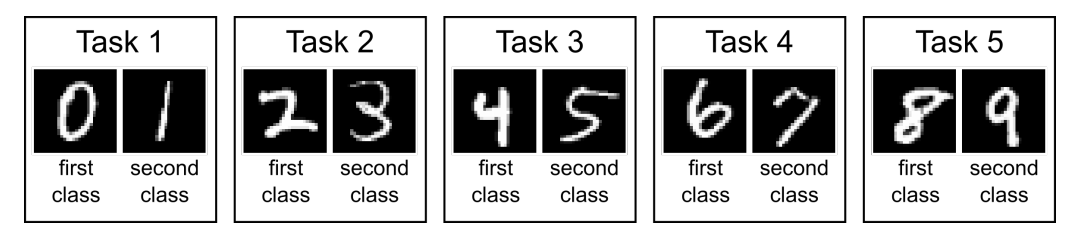
\includegraphics[width=0.9\textwidth]{Images/tasks_example_mnist.png}
    \caption{Schematic view of an MNIST task protocol, from \citep{van2019three}}
    \label{fig:mnistTaskProtocol}
\end{figure}


Looking at figure \ref{fig:mnistTaskProtocol} we can split MNIST according to the three scenarios as follows: 
\begin{table}[H]
\begin{tabularx}{0.9\textwidth}{l | X }
    \textbf{Scenario} & \textbf{Description} \\
     Task-incremental learning & With task given, is it the first or second class? (e.g. 0 or 1)  \\
     Domain-incremental learning & With task unknown, is it a first or second class? (e.g. in [0,2,4,6,8] or in [1,3,5,7,9]?\\
     Class-incremental learning & With task unknown, which digit is it? (e.g. choice from 0 to 9)

\end{tabularx}
     \caption{Split MNIST according to three scenarios from \citep{van2019three}}
     \label{tab:mnist_tasks}
\end{table}
The first scenario, Task-incremental learning (or Task-IL), involves an algorithm learning a set of distinct tasks sequentially, where the task identity is explicitly provided or clearly distinguishable. Models can be trained with task-specific components, or even use separate networks for each task. This approach avoids the problem of catastrophic forgetting (adapting to a different distribution usually leads to a significant decrease in the ability to capture the original ones \citep{wang2023comprehensive}) altogether \citep{ruvolo2013ella, masse2018alleviating}. But the main challenge is to effectively share the learnt representations while optimising the performance-complexity trade-off \citep{lopez2017gradient, vogelstein2020representation}. 

The second scenario, Domain-incremental learning (or Domain-IL) encompasses an algorithm's ability to learn a sequence of tasks characterised by the same underlying problem structure (same classes) but varying contextual and in input distributions \citep{ke2021classic, mirza2022efficient}. Unlike the first scenario, the algorithm is not explicitly informed about the task at the test time. However, the output space remains consistent between tasks, indicating generalisability to unseen tasks \citep{aljundi2017expert}. 
As explained in \citep{mirza2022efficient} domain-incremental learning can be used to learn the same set of objects (classes) over a variety of weather conditions (domains), while having access to the task-ID (current weather), this is illustrated in Figure \ref{fig:domain-incremental-weather}. 

\begin{figure}[H]
    \centering
    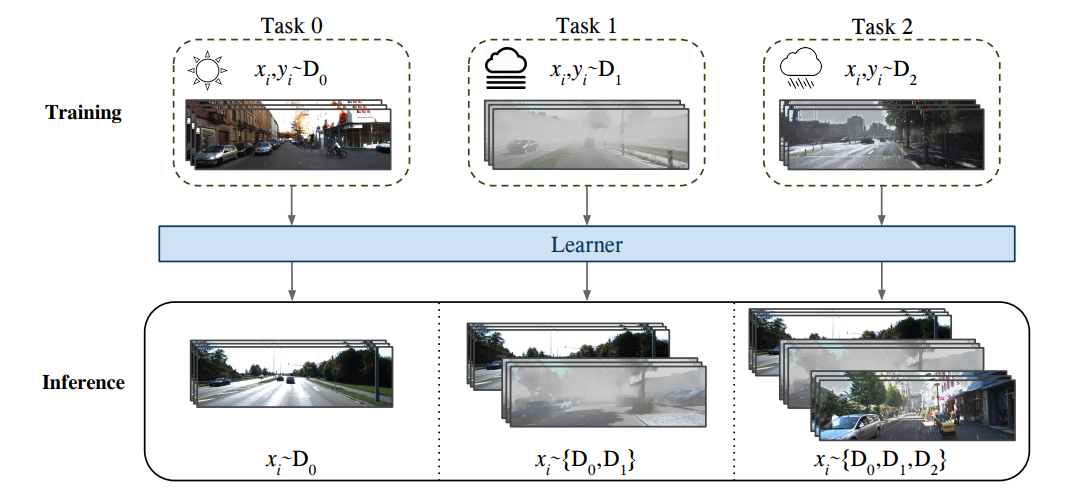
\includegraphics[width=0.9\textwidth]{Images/domain_incremental_weather.png}
    \caption{Domain-incremental learning setting. Different tasks correspond to different weather conditions which are learned in the training phase. During inference, the performance of the current task is evaluated along with all the previously seen tasks. \citep{mirza2022efficient}}
    \label{fig:domain-incremental-weather}
\end{figure}


The final scenario, Class-incremental learning (Class-IL), involves an algorithm learning to distinguish between a sequentially expanding set of classes or objects. The common setup involves encountering a sequence of classification tasks, where each task introduces new classes, and the algorithm must learn to classify samples across all accumulated classes \citep{von2019continual, van2020brain}. Task identification is crucial here as it determines the set of potential classes for a given sample. In essence, the algorithm must master both within-episode classification (distinguishing between classes in the same episode) and between-episode classification (identifying which episode a sample belongs to). This scenario presents a significant challenge to overcome catastrophic forgetting (see \ref{ref:subsub_catastrophic}), as the algorithm must not only maintain previously learned classes, but also adapt to new ones without degrading performance on previously learned classes \citep{belouadah2021comprehensive, masana2022class}. 

As illustrated in Figure \ref{fig:task-vs-class-il}, Task-IL involves having a task identifier available during inference, eliminating the need for methods to differentiate between classes from various tasks. On the other hand, in Class-IL, the learner does not have access to the task identifier during inference, requiring it to differentiate between all classes across tasks. 

\begin{figure}[H]
    \centering
    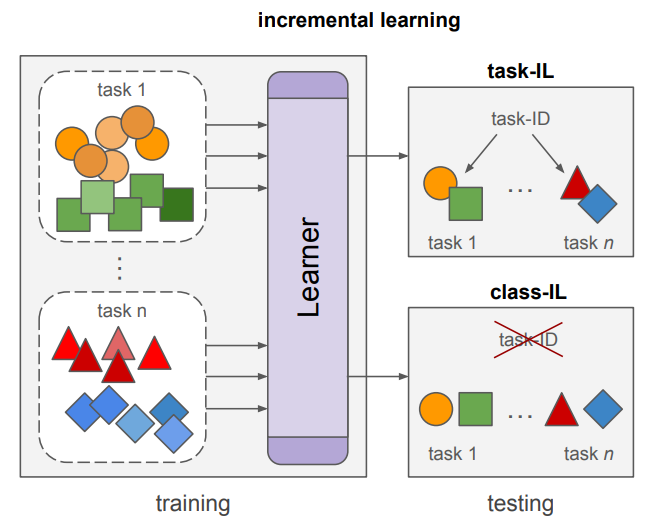
\includegraphics[width=0.6\textwidth]{Images/task_vs_class_il.png}
    \caption{In incremental learning, disjoint tasks are learned sequentially. Task-IL has access to the task identifier during evaluation, while class-IL does not. \citep{masana2022class}}
    \label{fig:task-vs-class-il}
\end{figure}

Empirical comparison of some \acrshort{dl} training strategies was executed on the MNIST \citep{deng2012mnist} and CIFAR-100 \citep{cifar} datasets. A baseline network with two fully connected hidden layers with a softmax output layer was used to compare performance.\\ 
The \acrshort{xdg} and the separate network methodology \citep{masse2018alleviating} require context knowledge of the training record, so they can only be applied in Task-IL scenarios. Regularisation methods such as \acrshort{ewc} \citep{kirkpatrick2017overcoming} employ a quadratic penalty term for each previously learnt context, effectively preventing parameter changes that would significantly deviate from the values acquired during context-specific training. 
Task-IL scenarios performed equally well as opposed to the baseline method, domain-IL and especially class-IL had a considerable drop in performance. The parameter regularisation implied a significant reduction. Replay-based algorithms had the best results for all scenarios of \acrshort{il}. \citep{khare2021unsupervised} found that the use of class imbalance improves detection in class-IL approaches.\\

\section{Background}
\label{sec:Background}
\subsection{CL Concepts and formulation}
\label{subsec:cl_concepts}
We follow the framework proposed by \citep{lesort2020continual}. 
In the context of continual learning, the data can be considered as coming from a (potentially infinite) sequence $\mathbf{D}$ of distributions that are not known in advance. This sequence, denoted as $\mathbf{D} = \{ D_{1}, ..., D_{N} \}$, is defined over the random variables $X$ and $Y$, where $X$ represents the input and $Y$ represents the output. At each time step $i$, the algorithm receives a training set $Tr_{i}$ consisting of one or more observations drawn from the distribution $D_{i}$. A learning task is marked by a distinct task label $t\in \{ 1,\dots,T\}$ and its intended goal or objective function $h^{*}$.

An algorithm with the signature $A^{CL}$, also known as a \acrlong{cl} algorithm, is defined as follows: \begin{equation} \label{eq:CL_algo} A_{i}^{CL} : \langle h_{i-1}, Tr_{i}, M_{i-1}, t_{i} \rangle \leftarrow \langle h_{i}, M_{i} \rangle \quad , \forall D_{i} \in \mathbf{D} \end{equation} In this equation, $h_i$ represents the current model or hypothesis that is continuously learned at time $i$. $M_{i}$ is an external memory buffer that stores previous training examples. $t_{i}$ is a task label associated with the training examples, and $Tr_{i}$ represents the training set of examples.

\acrshort{cl} methodologies are specific settings where the sequence of $N$ task labels follows a defined pattern over time. There are three commonly observed situations: \begin{itemize} \item Single Incremental Task (SIT): the task remains the same throughout. \item Multi Task (MT): each new task is different from the previous one. \item Multi Incremental Task (MIT): the model may encounter a combination of new and old tasks, which can be presented in an interleaved manner. \end{itemize} Task incremental scenarios assume that task labels are available for each sample. However, it is challenging to obtain explicit task labels for each sample in real-world applications \citep{cossu2021continual}.

The classification of \acrshort{cl} strategies can be categorised into three distinguishable groups: regularisation strategies, architectural strategies, and replay strategies \citep{parisi2019continual}. 

Regularisation strategies aim to achieve a balance between plasticity and stability by incorporating regularisation terms into the loss function. Example regularisation strategies are \acrshort{ewc} (see \ref{sec:ewc}), \acrshort{si} (see \ref{sec:si}) and \acrshort{lwf} (see \ref{sec:lwf}). 

The goal of a \acrshort{cl} algorithm is to learn how to accurately classify, at any specific training stage, examples from all of the observed tasks up until the current one $t\in \{ 1, \dots, t_{c} \}$:
\[
    \underset{\theta}{\mathrm{argmin}} \; \sum^{t_{c}}_{t=1} \mathbf{L}_{t}
\]
where
\[
    \mathbf{L}_{t} = \EX \left( L \left( y, f_{\theta} (x) \right) \right)
\]
and $\EX$ is the expectation over data sampled from a distribution $\mathbf{D}_t$. \\

\subsection{Catastrophic forgetting}
\label{ref:subsub_catastrophic}
While \acrshort{ml} models often achieve or even exceed human-level performance on specific tasks, they lack the ability to adapt dynamically to new data. Unlike humans, who learn concepts sequentially and reinforce their understanding by observing new examples, neural networks suffer from a phenomenon known as catastrophic forgetting \citep{french1999catastrophic}. This means that they need to be retrained from scratch every time new data becomes available. 
The dilemma (or trade-off) of Stability-Plasticity pertains to the capacity to incorporate new information while preserving past knowledge during the process of recoding \citep{grossberg2012studies}. Neural networks often tend to be skewed towards too much plasticity (integrating new knowledge) \citep{de2021continual}. Forgetting is, not only related to machines, it is part of the very nature of learning (e.g. forgetting biased information). The decay of forgetting can be described by a power law. When a person is taught a specific concept, if there is no repetition or emotional significance attached to it, the information is quickly forgotten but not entirely erased. Over time, forgetting follows a declining pattern \citep{pashler2009predicting}.


\subsection{CL training methods}
In the subsequent section, we will outline a few of the frequently employed training techniques. Most of the training strategies follow the guidelines of General Continual Learning (GCL) as proposed by \citep{farquhar2018towards}. 
\begin{itemize}
    \item Do not rely on task boundaries.
    \item No oracle with task identifiers during testing.
    \item A bounded constant memory throughout training.
\end{itemize}

\subsubsection{Elastic Weight Consolidation}
\label{sec:ewc}
The study by \citep{kirkpatrick2017overcoming} and \citep{de2021continual} explains \acrshort{ewc} is a regularization method designed to address the issue of catastrophic forgetting in neural networks. It achieves this by constraining the learning process. The main concept behind \acrshort{ewc} involves incorporating a quadratic penalty term into the standard loss function. This penalty term takes into account the difference between the current weight values and the optimal weights that were obtained during the previous task learning phase. By doing so, \acrshort{ewc} minimises interference between tasks and ensures a balance between learning new tasks and retaining knowledge from previous tasks.
\begin{figure}[h]
\centering
    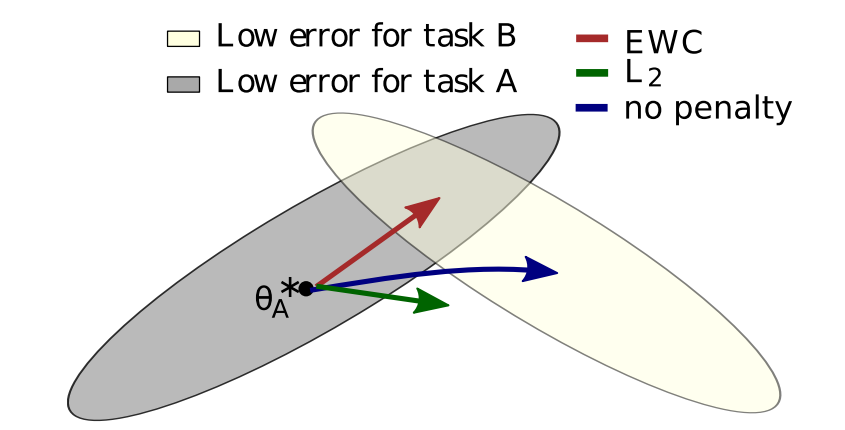
\includegraphics[width=0.7\textwidth]{Images//ewc.png}
    \caption{EWC guarantees task A is remembered while training on B. \citep{kirkpatrick2017overcoming}}
    \label{fig:ewc}
\end{figure}
The concept of Elastic Weight Consolidation (EWC) allows for the retention of knowledge from task A while training on task B. The training process is represented in a conceptual parameter space (Figure \ref{fig:ewc}), where regions of parameters resulting in good performance on task A are depicted in grey, and those for task B are depicted in cream color. Once task A is learned, the parameters are located at $\theta_{A}^{*}$ (see Figure \ref{fig:ewc}). However, when considering the gradient steps of task B (blue arrow in Figure \ref{fig:ewc}), the loss of task B is minimized but at the expense of compromising the knowledge acquired from task A, this is equivalent to "no penalty": \[ \theta^* = \underset{\theta}{\mathrm{argmin}} \, \mathbf{L}_B(\theta) \] To prevent forgetting the learned knowledge from task A, a distance minimization technique is applied between $\theta$ and $\theta^{*}_{A}$ ($L_{2}$ in Figure \ref{fig:ewc}): \[ \theta^{*} = \underset{\theta}{\mathrm{argmin}} \, \mathbf{L_B(\theta)} + \frac{1}{2} \alpha ( \theta - \theta_{A}^{*} )^{2} \] Here, $\alpha$ is a scalar that determines the relative importance of the old task compared to the new one. 
The constraint of $L_{2}$ is highly restrictive and has the capacity to hinder the learning process of task B. In the realm of deep learning, it is common practice to excessively parameterize models. Some parameters may be less beneficial while others hold greater significance.

\acrshort{ewc} discovers a solution for task B without significantly impairing task A's performance (red arrow in Figure \ref{fig:ewc}) by explicitly calculating the importance of each weight for task A. This importance value, also called the Fisher Information matrix\footnote{The Fisher Information Matrix provides a curvature approximation of the loss function \citep{ly2017tutorial}}, quantifies the weight's contribution to the performance on previously learned tasks. Weights with higher importance values have a greater impact on the performance of the previous tasks. The learning process is formulated as follows: 
\[
\theta^{*} = \underset{\theta}{\mathrm{argmin}} \; \mathbf{L_B}(\theta) + \frac{1}{2} \lambda I_{\theta_{A}^{*},i}(\theta_{i} - \theta_{A,i}^{*})^{2}
\]
In the above equation, $L_{\theta_{A}^{*},i}$ represents the diagonal elements of the Fischer information matrix, and $\lambda$ is the hyperparameter that determines the strength of the regularization penalty.
The implementation operates by computing the Fisher information matrix $I_{i}$ for each batch $B_{i}$. This is achieved by conducting a forward and backward propagation of the patterns. Subsequently, the implementation stores the obtained $I$ and the optimal weights $\theta$.


\subsubsection{Synaptic Intelligence}
\label{sec:si}
According to \citep{zenke2017continual} and \citep{maltoni2019continuous}, the introduction of \acrshort{si} as a modification to \acrshort{ewc} involved performing the computationally expensive Fisher matrix computations online during \acrshort{sgd} throughout the learning process. The implementation of this approach involves calculating the weight importance matrix $I_{i}$ for each batch of data samples $B_{i}$ using the information already available during \acrshort{sgd}. The weight importance matrix $I$ and the optimal weights $\theta$ are then stored.


\subsubsection{Learning without Forgetting}
\label{sec:lwf}
The aim of the \acrshort{lwf} approach is to manage the process of forgetting by enforcing output stability (Maltoni et al., 2019). It follows a similar approach to parameter regularization methods like EWC (see Section \ref{sec:ewc}) and SI (see Section \ref{sec:si}), where a regularization term is added to the classification loss function $\mathbf{L}$. Although originally designed for classification tasks, it has also been successfully utilized in 
object detection \citep{de2021continual}.


\subsubsection{FROMP}
\label{sec:fromp}
The \acrshort{fromp} training strategy is a novel approach in \acrshort{cl} addressing the catastrophic forgetting problem. It regularises the network outputs at a few memorable past examples that are crucial to avoid forgetting. By using a Gaussian process formulation of deep networks, the approach enables training in weight-space while identifying both the memorable past and a functional prior. It involves a slight modification of the Adam optimizer and a minor increase in computational cost. \citep{pan2020continual}. A schematic representation of \acrshort{fromp} is depicted in figure \ref{fig:fromp}. 
\begin{figure}
    \centering
    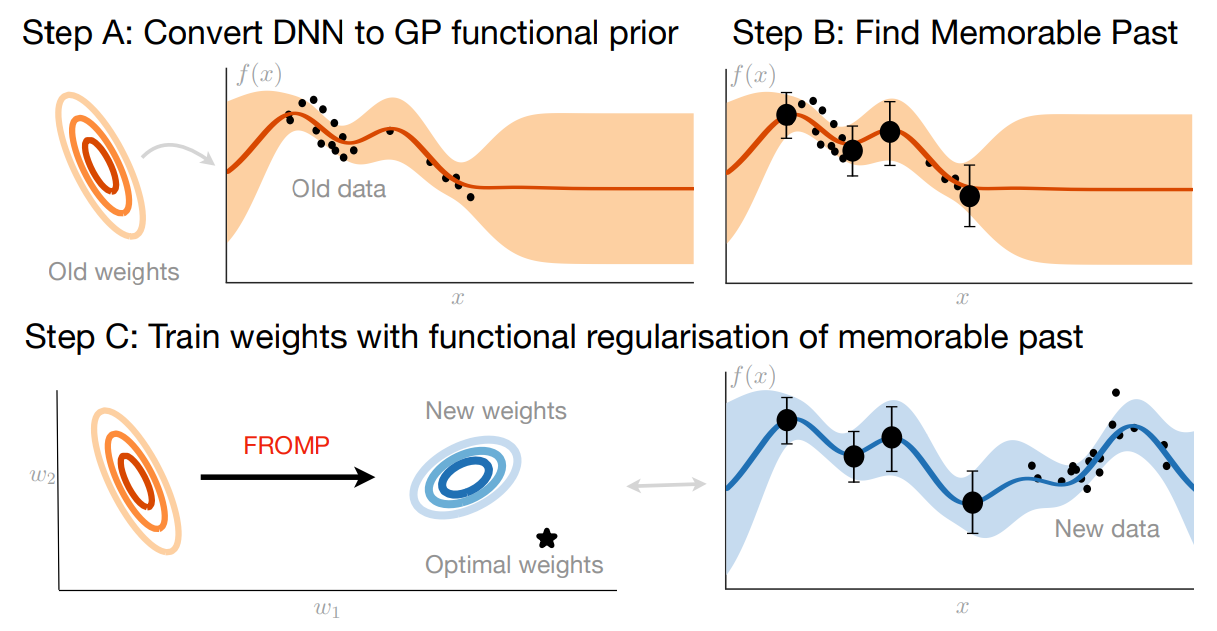
\includegraphics[width=0.8\textwidth]{Images//fromp.png}
    \caption{The FROMP method consists of three main steps where they first convert a DNN (Deep Neural Network) to a GP (Gaussian-Process), find memorable examples, and train weights with functional regularisation of those examples. \citep{pan2020continual}}
    \label{fig:fromp}
\end{figure}

\subsubsection{GEM}
\label{sec:gem}
The \acrlong{cl} (\acrshort{cl}) strategy, proposed by \citep{lopez2017gradient}, is a model that overcomes the limitations imposed by Empirical Risk Minimization \citep{vapnik1991principles} on other supervised learning techniques. To bridge this gap, the \acrlong{gem} (\acrshort{gem}) model incorporates an episodic memory $M_t$ that selectively stores a subset of observed examples from a specific task $t$. The memory capacity is limited to a total of $M$ locations, with each task having $m=\frac{M}{T}$ memories. The examples stored in $M$ are utilized to determine predictor functions $f_{\theta}$ by minimising the corresponding loss function
\[
\mathbf{L}(f_{\theta}, M_{k}) = \frac{1}{|M_{k}|} \sum_{(x_i, k, y_i) \in M_{k}} \mathbf{L}(f_{\theta}(x_i , k), y_i)
\]
Overfitting to the stored examples in $M_{k}$ is a common issue when minimizing the loss at the current example along with the above loss function. To address this problem, they solve the following optimization problem:
\[ 
\underset{\theta}{\mathrm{argmin }} \; \mathbf{L}(f_{\theta}(x,t),y) \text{ subject to } \mathbf{L}(f_{\theta}, M_{k}) \leq \mathbf{L}(f_{\theta}^{t-1}, m_k), \forall k<t 
\]
Here, $f^{t-1}_{\theta}$ represents the previous predictor state at the end of learning task $t-1$. The detailed solution can be found in the original paper by \citep{lopez2017gradient}.


\subsubsection{A-GEM}
\label{sec:a-gem}
\citep{chaudhry2018efficient} proposes a more efficient version of \acrshort{gem} where it tries to ensure that at every training step the average episodic memory loss over the previous tasks does not increase. Formally the objective of \acrshort{agem} is
\[ 
\underset{\theta}{\mathrm{argmin }} \; \mathbf{L}(f_{\theta} D_{t}) \text{ such that } \mathbf{L}(f_{\theta}, M) \leq \mathbf{L}(f_{\theta}^{t-1}, M), \text{ where } M = \underset{k<t}{\bigcup} M_{k} 
\]
The detailed solution and update rule can be found in the original paper by \citep{chaudhry2018efficient}.

\subsubsection{iCaRL}
As described in \citep{rebuffi2017icarl} iCaRL (Incremental Classifier and Representation Learning) allows learning in a class incremental way as depicted in figure \ref{fig:icarl}. It learns strong classifiers and a data representation simultaneously. In iCaRL, the model learns to recognize new classes while retaining its ability to recognize old ones. This is achieved by storing examples of each class, which are selected based on their closeness to the mean feature of that class. 
The model is then trained on both the new data and these examples. This approach ensures that the model does not forget the old classes when learning new ones. 

\begin{wrapfigure}{l}{0.40\textwidth}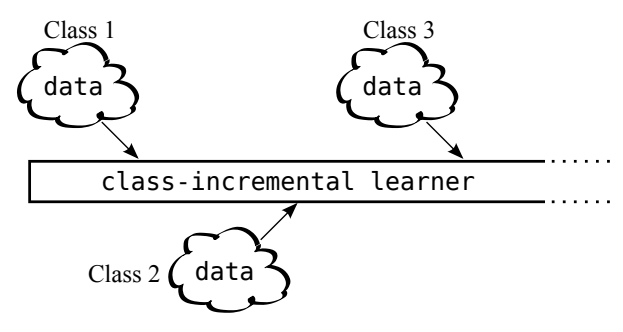
\includegraphics[width=0.45\textwidth]{Images//class_incremental_learning.png}
    \caption{Class-incremental learning. \citep{rebuffi2017icarl}}
    \label{fig:icarl}
\end{wrapfigure}


iCaRL utilizes a \acrshort{cnn} as its underlying mechanism. The \acrshort{cnn} functions as a feature extractor that can be trained, denoted as $\phi: X \rightarrow \mathbf{R}^{d}$, followed by a single classification layer containing sigmoid output nodes equal to the number of classes encountered up to that point. All feature vectors undergo $L^{2}$ normalization. The classification approach employed by iCaRL is based on a nearest-mean-of-exemplars strategy.\\
In order to predict a label, $y^{*}$, for a new input, $x$, the system calculates a prototype vector for each class seen so far, represented as $\mu_{1}, ..., \mu_{t}$, where $\mu_{y}$ represents the average feature vector of all examples belonging to class $y$. It also computes the feature vector of the image that should be classified and assigns the class label with the most similar prototype: 
\[
y^{*} = \underset{y=1,...,t}{\mathrm{argmin }} \| \phi(x) - \mu_{y} \|
\]

\subsubsection{SCR}
\label{sec:SCR}
\begin{wrapfigure}{r}{0.40\textwidth}
    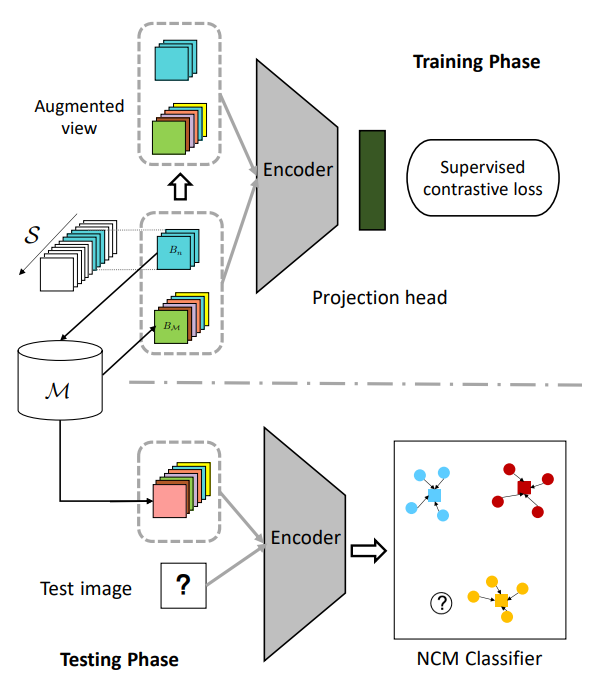
\includegraphics[width=0.40\textwidth]{Images/scr_architecture.png}
    \caption{A schematic view of SCR. \citep{mai2021supervised}}
    \label{fig:scr_architecture}
\end{wrapfigure}

\acrfull{scr} is a technique introduced by \citep{mai2021supervised} to address some challenges common in \acrshort{cl}. 
Because the softmax classifier is not the best choice for CL approaches, it aims to leverage the \acrfull{ncm} classifier instead to effectively mitigate catastrophic forgetting (or also called task-recency bias).\\
The \acrshort{scr} process (see Figure \ref{fig:scr_architecture}) involves the creation of an input batch during training by combining a minibatch $B_{n}$ from the datastream with another minibatch $B_{M}$ from the memory buffer $M_{i}$.\\ 
These input batches, along with their augmented views, are encoded by a shared encoder  and projection head. Followed by an evaluation using supervised contrastive loss. In the testing phase, the projection head is removed. Supervised Contrastive Loss is an alternative loss function to cross entropy that can leverage label information more effectively. \citep{khosla2020supervised}.

\subsubsection{DER and DER++}
\acrfull{der} is proposed by \citep{buzzega2020dark} as an improvement on Experience Replay (ER) while maintaining a simple formulation. It relies on dark knowledge for distilling past experiences, sampled over the training trajectory. \\
Formally, given a \acrshort{cl} classification split in $T$ tasks

It is problematic that the data from earlier tasks $\mathbf{D}_{t}$ for $t \in \{ 1, \dots, t_{c} - 1 \}$ is unavailable. To preserve the knowledge acquired previously, the subsequent objective function, which mirrors the teacher-student method, is minimized:

\[
\mathbf{L}_{t_{c}} + \alpha \sum_{t=1}^{t_{c}-1} \EX \left[ D_{KL} \left( f_{\theta_{t}^{*}}(x) \parallel f_{\theta}(x) \right) \right]
\]
where $\theta_{t}^{*}$ is the optimal set of parameters at the end of task $t$, $\alpha$ is a hyperparameter balancing the trade-off between the terms. 
$D_{KL}$ stands for the Kullback-Leibler divergence, a measure of how one probability distribution diverges from a second, expected probability distribution. It is commonly used to quantify how much knowledge from previous tasks is retained or lost when learning new tasks \citep{goodfellow2016deep}.\\
The above objective function requires having access to $\mathbf{D}_{t}$ for earlier tasks. To address this issue, a replay buffer $M_{t}$ is utilized to store previous experiences related to task $t$. Instead of preserving the actual labels $y$, the network logits (pre-activation outputs) $z \doteq h_{\theta_{t}}(x)$ are maintained. 
\[
\mathbf{L}_{t_{c}} + \alpha \sum_{t=1}^{t_{c}-1} \EX \left[ D_{KL} \left( \sigma(z) \parallel f_{\theta}(x) \right) \right]
\]
where $\sigma$ is the softmax function and $(x,z)$ are drawn from the replay buffer $M_{t}$. \\
\acrshort{der} uses reservoir sampling as defined by \citep{vitter1985random} to select $|M|$ random samples from the input stream, this way guaranteeing the same probability of being stored in the buffer without knowing the length in advance. This way the previous equation (with $\EX$ drawn from $M$) becomes:
\[
\mathbf{L}_{t_{c}} + \alpha \EX \left[ D_{KL} \left( \sigma(z) \parallel f_{\theta}(x) \right) \right]
\]

Given some basic assumptions, as mentioned in \citep{hinton2015distilling}, maximizing the KL divergence corresponds to minimizing the Euclidean distance among the logits. Consequently, the target function for \acrshort{der} is defined as
\[
\mathbf{L}_{t_{c}} + \alpha \EX \left[ \| z - h_{\theta}(x) \|^{2}_{2} \right]
\]

with $\EX$ being approximated by gradient computation on batches sampled from the replay buffer \citep{buzzega2020dark, boschini2022class}. \\
\acrshort{der++} adjusts the objective function by adding an additional balancing term $\beta$ on alternative 'buffer' data points

\[
\mathbf{L}_{t_{c}} + \alpha \EX \left[ \| z_{1} - h_{\theta}(x_{1}) \|^{2}_{2} \right] + \beta \EX \left[ \mathbf{L} \left( y_{2}, f_{\theta}(x_{2}) \right) \right]
\]

\acrshort{der++} collapses to \acrshort{der} when the coefficient $\beta=0$. \\
Experiment results, as described in \citep{buzzega2020dark} conclude that \acrshort{der} converges to more flat minima and to more calibrated networks. 

\subsection{CL metrics}
\label{sec:il_metrics}
Evaluation of learning tasks is a major part of research. As \citep{qu2021recent} indicates, not only the performance on new tasks, but also the amount of forgotten wisdom must be considered. We follow the notation used in \citep{diaz2018don, lopez2017gradient, chaudhry2018riemannian} to define the most popular metrics. \\
We denote $a_{q,p}$ as the accuracy on the separate test set of the task $p$ after \acrshort{il} of $q$ previous tasks, where $p\leq q$.

\subsubsection{Average accuracy ($A_{q}$)}
The metric $A_{q}$, as explained in \citep{wang2023comprehensive}, is utilized to assess the effectiveness of the \acrshort{il} model. It is calculated by averaging the accuracies obtained after learning a total of $q$ tasks. 
\begin{equation}
\label{metric:A_q}
    A_{q} = \frac{1}{q} \sum_{p=1}^{q} a_{q,p}
\end{equation}
This method is employed to assess the capacity to retain information from previous tasks while acquiring new knowledge.

\subsubsection{Average forgetting ($F_{q}$)}
The metric $F_{q}$, which is described in \citep{qu2021recent}, quantifies the amount of knowledge that is forgotten during the first $q-1$ tasks. It is calculated using the formula \begin{equation}
\label{metric:F_q}
    F_{q} = \frac{1}{q-1} \sum_{p=1}^{q-1} f_{p}^{q} 
\end{equation} 
where $f_{p}^{q}$ represents the knowledge forgotten for task $p$. This is determined by subtracting the remaining knowledge after learning $q$ tasks from the maximum knowledge obtained during the \acrshort{il} process. In eq. \ref{metric:F_q}, $f_{p}^{q}$ is calculated as follows: 
\begin{equation}
\label{metric:f_p_q}
  f_{p}^{q} = \max_{o \in \{ 1, ..., q-1\}} a_{o,p} - a_{q,p} , \forall p < q.
\end{equation}

\subsubsection{Intransigence ($I_{q}$)}
The metric called Intransigence (or learning plasticity) quantifies the extent to which \acrshort{cl} hinders a model from learning a new task in comparison to traditional batch learning. It is calculated as follows: 
\begin{equation}
\label{metric:I_q}
    I_{q} = a^{*}_{q} - q_{q,q}
\end{equation} 
In eq. \ref{metric:I_q}, $a^{*}_{q}$ represents the accuracy achieved on the test set of the $q^{\text{th}}$ task when batch learning is employed for all $q$ tasks \citep{chaudhry2018riemannian}.

\subsubsection{Backward transfer ($BWT_{q}$)}
The concept of backward transfer, as described in \citep{lopez2017gradient}, is how much the learning process on task $q$ affects the performance of previously learned tasks. This can be quantified using the following equation: \begin{equation}
\label{metric:BWT_q}
BWT_{q} = \frac{1}{q-1} \sum_{p=1}^{q-1} (a_{q,p} - a_{p,p})
\end{equation}

\subsubsection{Forward transfer ($FWT_{q}$)}
Forward transfer refers to the degree to which the continuous learning of the $q^{\text{th}}$ task has the potential to influence the performance of future tasks. In \citep{lopez2017gradient}, the accuracy on the test set of the $p^{\text{th}}$ task at random initialization is represented as $b_{p}$. The forward transfer metric, denoted as $FWT_{q}$, is defined as follows: \begin{equation} FWT_{q} = \frac{1}{q-1} \sum_{p=2}^{q} (a_{p-1,p} - b_{p}) \end{equation}
\citep{wang2023comprehensive}test

\subsection{Python packages}
A recent toolbox called \verb|PyCIL| \citep{zhou2023class, zhou2023pycil} implements several state-of-the-art \acrshort{il} algorithms. The package \verb|Avalanche| \citep{lomonaco2021avalanche} provides a library for benchmarking, training, prototyping, training and evaluation of \acrshort{cl} algorithms. Continuum \citep{douillardlesort2021continuum} is a library that provides data loading functionalities for \acrshort{cl}. 

\subsubsection{Avalanche}
\label{sec:avalanche}
The Avalanche package came into existence with a clear goal in mind, \textit{"Pushing Continual Learning to the next level, providing a shared and collaborative library for fast prototyping, training and reproducible evaluation of continual learning algorithms."} \citep{avalancheContinualAIFiveMinutes}

Avalanche is structured based on a series of core design principles: 1) minimizing code length for rapid prototyping and error minimization, 2) ensuring reproducibility, 3) promoting modularity and reusability, 4) enhancing code efficiency, scalability, and portability and 5) prioritizing usability.


\begin{figure}[H]
    \centering
    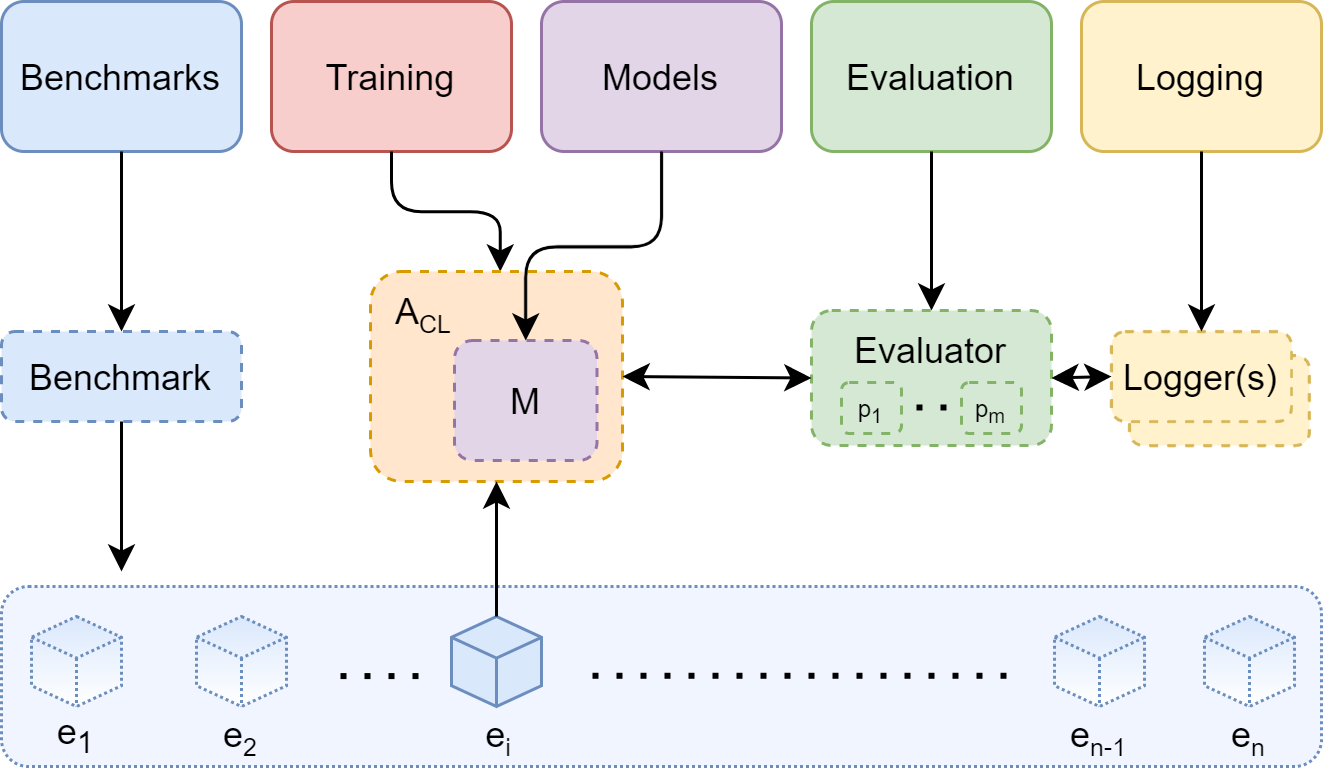
\includegraphics{Images//avalanche.png}
    \caption{The main Avalanche modules and how they interact with each other. \citep{avalancheContinualAIFiveMinutes} }
    \label{fig:avalanche}
\end{figure}
Avalanche is organized in five main modules denoted in figure \ref{fig:avalanche}. 

1) \textbf{Benchmarks}: This component preserves a consistent application programming interface (API) for managing data, primarily by producing a sequence of data from multiple datasets. It contains the primary \acrshort{cl} performance metrics (similar to the approach taken in \verb|torchvision| ).

2) \textbf{Training}: This module offers a comprehensive range of tools related to model training. It encompasses straightforward and effective methods for incorporating new continual learning strategies, along with a collection of pre-implemented \acrshort{cl} baselines and cutting-edge algorithms that can be utilized for comparison purposes.

3) \textbf{Evaluation}: This module offers a comprehensive set of tools and measurements that can help evaluate a \acrshort{cl} algorithm in relation to the various factors that we consider crucial for a system that learns continuously.

4) \textbf{Models}: In this module, you will discover various model structures and pre-trained models suitable for your ongoing learning experiment (similar to what has been done in \verb|torchvision.models|).

5) \textbf{Logging}: It contains sophisticated logging and visualization functionalities, such as built-in support for \verb|stdout|, file, and \verb|Tensorboard| (Effortlessly monitor your experiment metrics in real-time using just one line of code on a comprehensive interactive dashboard). 

\citep{lomonaco2021avalanche, carta2023avalanche}

\subsection{Saliency Mapping}
The Image-Specific Class Saliency Visualisation is a method described in \citep{simonyan2013deep} for understanding a \acrshort{cnn} decision-making process by visualizing the spatial support of a particular class within a given image. The goal is to rank the pixels of an input image based on their influence on the score function, which indicates the likelihood of the presence of a specific class.
Given an image $I_{0}$, a class label $c$ and a \acrshort{cnn} classifying score function $S_{c}(I_{0})$, we would like to rank the pixels of $I$ based on their influence on the score $S_{c}(I)$. 
The linear score model, where the score $S_{c}$ is determined by the dot product between the weight vector $w_{c}$ and the image $I$, and adding a bias term $b_{c}$. 
\[
S_{c}(I) = w_{c}^{T} I + b_{c}
\]
In this model, the importance of individual pixels in the image for the class $c$ is directly proportional to the magnitude of the corresponding elements in the weight vector $w_{c}$. However, the class score function is non-linear, therfore the linear model cannot be applied. 
The purpose of the Class Saliency Visualisation is to address this non-linearity in \acrshort{cnn}'s. Given an image $I_{0}$, the class score $S_{c}(I)$ can be approximated with a first-order Taylor expansion: 
\[
S_{c}(I) \approx w^{T} I + b
\]
where $w$ is the partial derivative of $S_{c}$ w.r.t. the image $I$ at the point $I_{0}$: 
\[
w = \left. \frac{\partial S_{c}}{\partial I} \right|_{I_{0}}
\]
The above approach aims to infer the importance of pixels in an image for a specific class despite the non-linear nature of the classifier. This visualization method helps in understanding how the model makes its predictions by highlighting which parts of the image contribute most significantly to the classification of a particular class. 

The class saliency map $M\in \mathbf{R}^{m\times n}$ for an image $I_{0}$ (of size $m\times n$) and a class $c$ requires a single back-propagation pass through the classification \acrshort{cnn}. The elements of the derivative $w$ are then rearranged. 

In case of a grey-scale image, the mapping is computed as $M_{ij} = \left| w_{h(i,j)} \right|$ where $h(i,j)$ is the corresponding pixel-index of $w$ in row $i$ and column $j$. 

In case the image is an RGB-image, the color channel $c$ must be taken into account. The authors \citep{simonyan2013deep} opt for the maximum value of $w$ over the different color channels: $M_{ij} = \max_{c} \left| w_{h(i,j,c)}\right|$

\begin{figure}
    \centering
    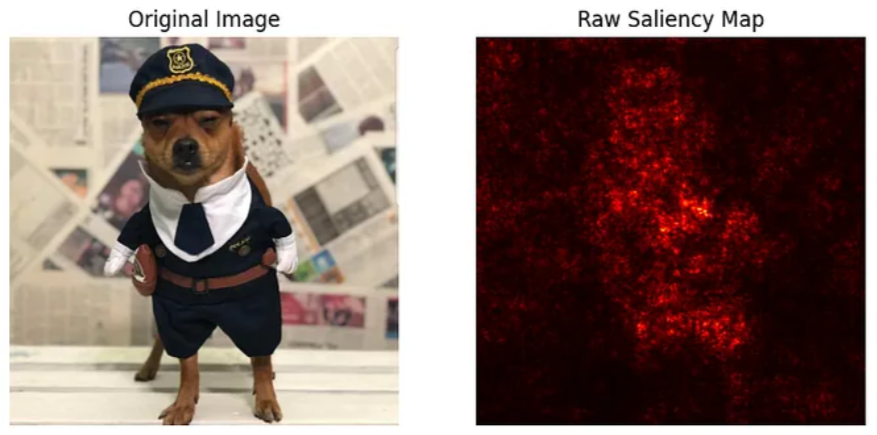
\includegraphics[width=0.6\textwidth]{Grad Assignment/Images/saliency_example.png}
    \caption{Example saliency map and original image. Taken from \citep{newginsam2024}}
    \label{fig:saliency_example}
\end{figure}




